% Options for packages loaded elsewhere
\PassOptionsToPackage{unicode}{hyperref}
\PassOptionsToPackage{hyphens}{url}
%
\documentclass[
  12pt,
]{article}
\usepackage{amsmath,amssymb}
\usepackage{lmodern}
\usepackage{ifxetex,ifluatex}
\ifnum 0\ifxetex 1\fi\ifluatex 1\fi=0 % if pdftex
  \usepackage[T1]{fontenc}
  \usepackage[utf8]{inputenc}
  \usepackage{textcomp} % provide euro and other symbols
\else % if luatex or xetex
  \usepackage{unicode-math}
  \defaultfontfeatures{Scale=MatchLowercase}
  \defaultfontfeatures[\rmfamily]{Ligatures=TeX,Scale=1}
\fi
% Use upquote if available, for straight quotes in verbatim environments
\IfFileExists{upquote.sty}{\usepackage{upquote}}{}
\IfFileExists{microtype.sty}{% use microtype if available
  \usepackage[]{microtype}
  \UseMicrotypeSet[protrusion]{basicmath} % disable protrusion for tt fonts
}{}
\makeatletter
\@ifundefined{KOMAClassName}{% if non-KOMA class
  \IfFileExists{parskip.sty}{%
    \usepackage{parskip}
  }{% else
    \setlength{\parindent}{0pt}
    \setlength{\parskip}{6pt plus 2pt minus 1pt}}
}{% if KOMA class
  \KOMAoptions{parskip=half}}
\makeatother
\usepackage{xcolor}
\IfFileExists{xurl.sty}{\usepackage{xurl}}{} % add URL line breaks if available
\IfFileExists{bookmark.sty}{\usepackage{bookmark}}{\usepackage{hyperref}}
\hypersetup{
  pdftitle={ADA2: Class 14, Ch 07b, Analysis of Covariance},
  pdfauthor={Name Here},
  hidelinks,
  pdfcreator={LaTeX via pandoc}}
\urlstyle{same} % disable monospaced font for URLs
\usepackage[margin=0.25in]{geometry}
\usepackage{color}
\usepackage{fancyvrb}
\newcommand{\VerbBar}{|}
\newcommand{\VERB}{\Verb[commandchars=\\\{\}]}
\DefineVerbatimEnvironment{Highlighting}{Verbatim}{commandchars=\\\{\}}
% Add ',fontsize=\small' for more characters per line
\usepackage{framed}
\definecolor{shadecolor}{RGB}{248,248,248}
\newenvironment{Shaded}{\begin{snugshade}}{\end{snugshade}}
\newcommand{\AlertTok}[1]{\textcolor[rgb]{0.94,0.16,0.16}{#1}}
\newcommand{\AnnotationTok}[1]{\textcolor[rgb]{0.56,0.35,0.01}{\textbf{\textit{#1}}}}
\newcommand{\AttributeTok}[1]{\textcolor[rgb]{0.77,0.63,0.00}{#1}}
\newcommand{\BaseNTok}[1]{\textcolor[rgb]{0.00,0.00,0.81}{#1}}
\newcommand{\BuiltInTok}[1]{#1}
\newcommand{\CharTok}[1]{\textcolor[rgb]{0.31,0.60,0.02}{#1}}
\newcommand{\CommentTok}[1]{\textcolor[rgb]{0.56,0.35,0.01}{\textit{#1}}}
\newcommand{\CommentVarTok}[1]{\textcolor[rgb]{0.56,0.35,0.01}{\textbf{\textit{#1}}}}
\newcommand{\ConstantTok}[1]{\textcolor[rgb]{0.00,0.00,0.00}{#1}}
\newcommand{\ControlFlowTok}[1]{\textcolor[rgb]{0.13,0.29,0.53}{\textbf{#1}}}
\newcommand{\DataTypeTok}[1]{\textcolor[rgb]{0.13,0.29,0.53}{#1}}
\newcommand{\DecValTok}[1]{\textcolor[rgb]{0.00,0.00,0.81}{#1}}
\newcommand{\DocumentationTok}[1]{\textcolor[rgb]{0.56,0.35,0.01}{\textbf{\textit{#1}}}}
\newcommand{\ErrorTok}[1]{\textcolor[rgb]{0.64,0.00,0.00}{\textbf{#1}}}
\newcommand{\ExtensionTok}[1]{#1}
\newcommand{\FloatTok}[1]{\textcolor[rgb]{0.00,0.00,0.81}{#1}}
\newcommand{\FunctionTok}[1]{\textcolor[rgb]{0.00,0.00,0.00}{#1}}
\newcommand{\ImportTok}[1]{#1}
\newcommand{\InformationTok}[1]{\textcolor[rgb]{0.56,0.35,0.01}{\textbf{\textit{#1}}}}
\newcommand{\KeywordTok}[1]{\textcolor[rgb]{0.13,0.29,0.53}{\textbf{#1}}}
\newcommand{\NormalTok}[1]{#1}
\newcommand{\OperatorTok}[1]{\textcolor[rgb]{0.81,0.36,0.00}{\textbf{#1}}}
\newcommand{\OtherTok}[1]{\textcolor[rgb]{0.56,0.35,0.01}{#1}}
\newcommand{\PreprocessorTok}[1]{\textcolor[rgb]{0.56,0.35,0.01}{\textit{#1}}}
\newcommand{\RegionMarkerTok}[1]{#1}
\newcommand{\SpecialCharTok}[1]{\textcolor[rgb]{0.00,0.00,0.00}{#1}}
\newcommand{\SpecialStringTok}[1]{\textcolor[rgb]{0.31,0.60,0.02}{#1}}
\newcommand{\StringTok}[1]{\textcolor[rgb]{0.31,0.60,0.02}{#1}}
\newcommand{\VariableTok}[1]{\textcolor[rgb]{0.00,0.00,0.00}{#1}}
\newcommand{\VerbatimStringTok}[1]{\textcolor[rgb]{0.31,0.60,0.02}{#1}}
\newcommand{\WarningTok}[1]{\textcolor[rgb]{0.56,0.35,0.01}{\textbf{\textit{#1}}}}
\usepackage{graphicx}
\makeatletter
\def\maxwidth{\ifdim\Gin@nat@width>\linewidth\linewidth\else\Gin@nat@width\fi}
\def\maxheight{\ifdim\Gin@nat@height>\textheight\textheight\else\Gin@nat@height\fi}
\makeatother
% Scale images if necessary, so that they will not overflow the page
% margins by default, and it is still possible to overwrite the defaults
% using explicit options in \includegraphics[width, height, ...]{}
\setkeys{Gin}{width=\maxwidth,height=\maxheight,keepaspectratio}
% Set default figure placement to htbp
\makeatletter
\def\fps@figure{htbp}
\makeatother
\setlength{\emergencystretch}{3em} % prevent overfull lines
\providecommand{\tightlist}{%
  \setlength{\itemsep}{0pt}\setlength{\parskip}{0pt}}
\setcounter{secnumdepth}{-\maxdimen} % remove section numbering
\usepackage{booktabs}
\usepackage{longtable}
\usepackage{array}
\usepackage{multirow}
\usepackage{wrapfig}
\usepackage{float}
\usepackage{colortbl}
\usepackage{pdflscape}
\usepackage{tabu}
\usepackage{threeparttable}
\usepackage{threeparttablex}
\usepackage[normalem]{ulem}
\usepackage{makecell}
\usepackage{xcolor}
\ifluatex
  \usepackage{selnolig}  % disable illegal ligatures
\fi

\title{ADA2: Class 14, Ch 07b, Analysis of Covariance}
\author{Name Here}
\date{March 10, 2022}

\begin{document}
\maketitle

This is a challenging dataset, in part because it's real and messy. I
will guide you through a simplified sensible analysis, but other models
are possible.

\emph{Note that I needed to set \texttt{cache=FALSE} to assure all
output was updated.}

\hypertarget{ancova-model-albuquerque-nm-87108-house-and-apartment-listing-prices}{%
\section{ANCOVA model: Albuquerque NM 87108, House and Apartment listing
prices}\label{ancova-model-albuquerque-nm-87108-house-and-apartment-listing-prices}}

Prof Erhardt constructed a dataset of listing prices for dwellings
(homes and apartments) for sale from
\href{http://www.zillow.com/homes/for_sale/Albuquerque-NM-87108/95303_rid/any_days/35.095087-106.52167835.035021-106.633258_rect/13_zm/0_mmm/}{Zillow.com}
on Feb 26, 2016 at 1 PM for Albuquerque NM 87108. In this assignment
we'll develop a model to help understand which qualities that contribute
to a \textbf{typical dwelling's listing price}. We will then also
predict the listing prices of new listings posted on the following day,
Feb 27, 2016 by 2 PM.

Because we want to model a \emph{typical dwelling}, it is completely
reasonable to remove ``unusual'' dwellings from the dataset. Dwellings
have a distribution with a
\href{https://en.wikipedia.org/wiki/Long_tail}{long tail}!

\hypertarget{unusual-assignment-not-top-down-but-up-down-up-down}{%
\subsection{Unusual assignment, not top-down, but
up-down-up-down}\label{unusual-assignment-not-top-down-but-up-down-up-down}}

This is an unusual assignment because the workflow of this assignment
isn't top-down; instead, you'll be scrolling up and down as you make
decisions about the data and model you're fitting. Yes, I have much of
the code worked out for you. However, there are data decisions to make
early in the code (such as excluding observations, transforming
variables, etc.) that depend on the analysis (model checking) later.
Think of it as a ``choose your own adventure'' that I've written for
you.

\hypertarget{keep-a-record-of-your-decisions}{%
\subsubsection{Keep a record of your
decisions}\label{keep-a-record-of-your-decisions}}

It is always desirable to make your work reproducible, either by someone
else or by your future self. For each step you take, keep a diary of (a)
what the next minor goal is, (b) what evidence/information you have, (c)
what decision you make, and (d) what the outcome was.

For example, here's the first couple steps of your diary:

\begin{enumerate}
\def\labelenumi{\arabic{enumi}.}
\tightlist
\item
  Include only ``typical dwellings''. Based on scatterplot, remove
  extreme observations. Keep only HOUSE and APARTMENT.
\item
  Exclude a few variables to reduce multicollinearity between predictor
  variables. Exclude \texttt{Baths} and \texttt{LotSize}.d
\item
  etc.
\end{enumerate}

\hypertarget{p-step-1-restrict-data-to-typical-dwellings}{%
\subsection{\texorpdfstring{\textbf{(2 p)} (Step 1) Restrict data to
``typical''
dwellings}{(2 p) (Step 1) Restrict data to ``typical'' dwellings}}\label{p-step-1-restrict-data-to-typical-dwellings}}

\textbf{Step 1:} After looking at the scatterplot below, identify what
you consider to be a ``typical dwelling'' and exclude observations far
from that range. For example, there are only a couple \texttt{TypeSale}
that are common enough to model; remember to run \texttt{factor()} again
to remove factor levels that no longer appear.

\begin{Shaded}
\begin{Highlighting}[]
\FunctionTok{library}\NormalTok{(erikmisc)}
\FunctionTok{library}\NormalTok{(tidyverse)}
\FunctionTok{library}\NormalTok{(car)}

\CommentTok{\# First, download the data to your computer,}
\CommentTok{\#   save in the same folder as this Rmd file.}

\CommentTok{\# read the data, skip the first two comment lines of the data file}
\NormalTok{dat\_abq }\OtherTok{\textless{}{-}}
  \FunctionTok{read\_csv}\NormalTok{(}\StringTok{"\textasciitilde{}/Dropbox/3\_Education/Courses/stat\_528\_ada2/ADA2\_CL\_14\_HomePricesZillow\_Abq87108.csv"}\NormalTok{, }\AttributeTok{skip=}\DecValTok{2}\NormalTok{) }\SpecialCharTok{\%\textgreater{}\%}
  \FunctionTok{mutate}\NormalTok{(}
    \AttributeTok{id =} \DecValTok{1}\SpecialCharTok{:}\FunctionTok{n}\NormalTok{()}
\NormalTok{  , }\AttributeTok{TypeSale =} \FunctionTok{factor}\NormalTok{(TypeSale)}
    \CommentTok{\# To help scale the intercept to a more reasonable value}
    \CommentTok{\#   Scaling the x{-}variables are sometimes done to the mean of each x.}
    \CommentTok{\# center year at 1900 (negative values are older, {-}10 is built in 1890)}
\NormalTok{  , }\AttributeTok{YearBuilt\_1900 =}\NormalTok{ YearBuilt }\SpecialCharTok{{-}} \DecValTok{1900}
\NormalTok{  , }\AttributeTok{logPriceList =} \FunctionTok{log}\NormalTok{(PriceList, }\DecValTok{10}\NormalTok{)}
\NormalTok{  , }\AttributeTok{logSizeSqft =} \FunctionTok{log}\NormalTok{(Size\_sqft, }\DecValTok{10}\NormalTok{)}
\NormalTok{  ) }\SpecialCharTok{\%\textgreater{}\%}
  \FunctionTok{select}\NormalTok{(}
\NormalTok{    id, }\FunctionTok{everything}\NormalTok{()}
\NormalTok{    , }\SpecialCharTok{{-}}\NormalTok{Address, }\SpecialCharTok{{-}}\NormalTok{YearBuilt}
\NormalTok{  )}

\FunctionTok{head}\NormalTok{(dat\_abq)}
\end{Highlighting}
\end{Shaded}

\begin{tabular}{r|l|r|r|r|r|r|r|r|r|r}
\hline
id & TypeSale & PriceList & Beds & Baths & Size\_sqft & LotSize & DaysListed & YearBuilt\_1900 & logPriceList & logSizeSqft\\
\hline
1 & HOUSE & 186900 & 3 & 2 & 1305 & 6969 & 0 & 54 & 5.271609 & 3.115610\\
\hline
2 & APARTMENT & 305000 & 1 & 1 & 2523 & 6098 & 0 & 48 & 5.484300 & 3.401917\\
\hline
3 & APARTMENT & 244000 & 1 & 1 & 2816 & 6098 & 0 & 89 & 5.387390 & 3.449633\\
\hline
4 & CONDO & 108000 & 3 & 2 & 1137 & NA & 0 & 96 & 5.033424 & 3.055760\\
\hline
5 & CONDO & 64900 & 2 & 1 & 1000 & NA & 1 & 85 & 4.812245 & 3.000000\\
\hline
6 & HOUSE & 275000 & 3 & 3 & 2022 & 6098 & 1 & 52 & 5.439333 & 3.305781\\
\hline
\end{tabular}

\begin{Shaded}
\begin{Highlighting}[]
\DocumentationTok{\#\# RETURN HERE TO SUBSET THE DATA}

\NormalTok{dat\_abq }\OtherTok{\textless{}{-}}
\NormalTok{  dat\_abq }\SpecialCharTok{\%\textgreater{}\%}
  \FunctionTok{filter}\NormalTok{(}
\NormalTok{    TypeSale }\SpecialCharTok{\%in\%} \FunctionTok{c}\NormalTok{(}\StringTok{"APARTMENT"}\NormalTok{, }\StringTok{"HOUSE"}\NormalTok{), }
\NormalTok{    PriceList }\SpecialCharTok{\textless{}} \FloatTok{6e5}
\NormalTok{  ) }\SpecialCharTok{\%\textgreater{}\%}
  \FunctionTok{mutate}\NormalTok{(}\FunctionTok{across}\NormalTok{(TypeSale, }\SpecialCharTok{\textasciitilde{}}\FunctionTok{factor}\NormalTok{(TypeSale))) }\SpecialCharTok{\%\textgreater{}\%}
  \FunctionTok{select}\NormalTok{(}\SpecialCharTok{{-}}\FunctionTok{c}\NormalTok{(Baths, LotSize))}
\CommentTok{\# note, if you remove a level from a categorical variable, then run factor() again}

  \CommentTok{\# SOLUTION}
  \CommentTok{\# these deletions are based only on the scatter plot in order to have}
  \CommentTok{\#  "typical" dwellings}

\FunctionTok{str}\NormalTok{(dat\_abq)}
\end{Highlighting}
\end{Shaded}

\begin{verbatim}
tibble [129 x 9] (S3: tbl_df/tbl/data.frame)
 $ id            : int [1:129] 1 2 3 6 7 9 10 12 13 14 ...
 $ TypeSale      : Factor w/ 2 levels "APARTMENT","HOUSE": 2 1 1 2 2 2 2 1 2 2 ...
 $ PriceList     : num [1:129] 186900 305000 244000 275000 133000 ...
 $ Beds          : num [1:129] 3 1 1 3 2 3 3 1 4 2 ...
 $ Size_sqft     : num [1:129] 1305 2523 2816 2022 1440 ...
 $ DaysListed    : num [1:129] 0 0 0 1 1 1 2 2 6 6 ...
 $ YearBuilt_1900: num [1:129] 54 48 89 52 52 58 52 49 41 53 ...
 $ logPriceList  : num [1:129] 5.27 5.48 5.39 5.44 5.12 ...
 $ logSizeSqft   : num [1:129] 3.12 3.4 3.45 3.31 3.16 ...
\end{verbatim}

\begin{Shaded}
\begin{Highlighting}[]
\FunctionTok{table}\NormalTok{(dat\_abq}\SpecialCharTok{$}\NormalTok{TypeSale)}
\end{Highlighting}
\end{Shaded}

\begin{verbatim}
APARTMENT     HOUSE 
       40        89 
\end{verbatim}

\begin{Shaded}
\begin{Highlighting}[]
\NormalTok{dat\_abq }\SpecialCharTok{\%\textgreater{}\%}
  \FunctionTok{ggplot}\NormalTok{() }\SpecialCharTok{+} 
  \FunctionTok{geom\_histogram}\NormalTok{(}\FunctionTok{aes}\NormalTok{(}\AttributeTok{x =}\NormalTok{ logPriceList))}
\end{Highlighting}
\end{Shaded}

\begin{center}\includegraphics{ADA2_CL_14_ANCOVA_AbqHomePrices_files/figure-latex/unnamed-chunk-2-1} \end{center}

\hypertarget{p-step-3-transform-response-if-necessary.}{%
\subsection{\texorpdfstring{\textbf{(2 p)} (Step 3) Transform response,
if
necessary.}{(2 p) (Step 3) Transform response, if necessary.}}\label{p-step-3-transform-response-if-necessary.}}

\textbf{Step 3:} Does the response variable require a transformation? If
so, what transformation is recommended from the model diagnostic plots
(Box-Cox)?

\hypertarget{solution}{%
\subsubsection{Solution}\label{solution}}

\begin{Shaded}
\begin{Highlighting}[]
\NormalTok{dat\_abq }\OtherTok{\textless{}{-}}
\NormalTok{  dat\_abq }\SpecialCharTok{\%\textgreater{}\%}
  \FunctionTok{mutate}\NormalTok{(}
    \CommentTok{\# Price in units of $1000}
    \AttributeTok{PriceListK =}\NormalTok{ PriceList }\SpecialCharTok{/} \DecValTok{1000}

    \CommentTok{\# SOLUTION}
\NormalTok{  ) }\SpecialCharTok{\%\textgreater{}\%}
  \FunctionTok{select}\NormalTok{(}
    \SpecialCharTok{{-}}\NormalTok{PriceList}
\NormalTok{  )}

\FunctionTok{str}\NormalTok{(dat\_abq)}
\end{Highlighting}
\end{Shaded}

\begin{verbatim}
tibble [129 x 9] (S3: tbl_df/tbl/data.frame)
 $ id            : int [1:129] 1 2 3 6 7 9 10 12 13 14 ...
 $ TypeSale      : Factor w/ 2 levels "APARTMENT","HOUSE": 2 1 1 2 2 2 2 1 2 2 ...
 $ Beds          : num [1:129] 3 1 1 3 2 3 3 1 4 2 ...
 $ Size_sqft     : num [1:129] 1305 2523 2816 2022 1440 ...
 $ DaysListed    : num [1:129] 0 0 0 1 1 1 2 2 6 6 ...
 $ YearBuilt_1900: num [1:129] 54 48 89 52 52 58 52 49 41 53 ...
 $ logPriceList  : num [1:129] 5.27 5.48 5.39 5.44 5.12 ...
 $ logSizeSqft   : num [1:129] 3.12 3.4 3.45 3.31 3.16 ...
 $ PriceListK    : num [1:129] 187 305 244 275 133 ...
\end{verbatim}

\begin{Shaded}
\begin{Highlighting}[]
\NormalTok{mod1 }\OtherTok{\textless{}{-}} \FunctionTok{lm}\NormalTok{(logPriceList }\SpecialCharTok{\textasciitilde{}}\NormalTok{ Beds }\SpecialCharTok{+}\NormalTok{ Size\_sqft }\SpecialCharTok{+}\NormalTok{ DaysListed }\SpecialCharTok{+}\NormalTok{ YearBuilt\_1900, }
           \AttributeTok{data =}\NormalTok{ dat\_abq)}
\FunctionTok{boxCox}\NormalTok{(mod1)}
\end{Highlighting}
\end{Shaded}

\begin{center}\includegraphics{ADA2_CL_14_ANCOVA_AbqHomePrices_files/figure-latex/unnamed-chunk-4-1} \end{center}

The log transformation is clearly supported by the Box-Cox profile.

\hypertarget{p-step-4-remove-extremely-influential-observations.}{%
\subsection{\texorpdfstring{\textbf{(2 p)} (Step 4) Remove extremely
influential
observations.}{(2 p) (Step 4) Remove extremely influential observations.}}\label{p-step-4-remove-extremely-influential-observations.}}

\textbf{Step 4:} The goal is to develop a model that will work well for
the typical dwellings. If an observation is highly influential, then
it's unusual.

\begin{Shaded}
\begin{Highlighting}[]
\FunctionTok{e\_plot\_lm\_diagostics}\NormalTok{(mod1)}
\end{Highlighting}
\end{Shaded}

\begin{center}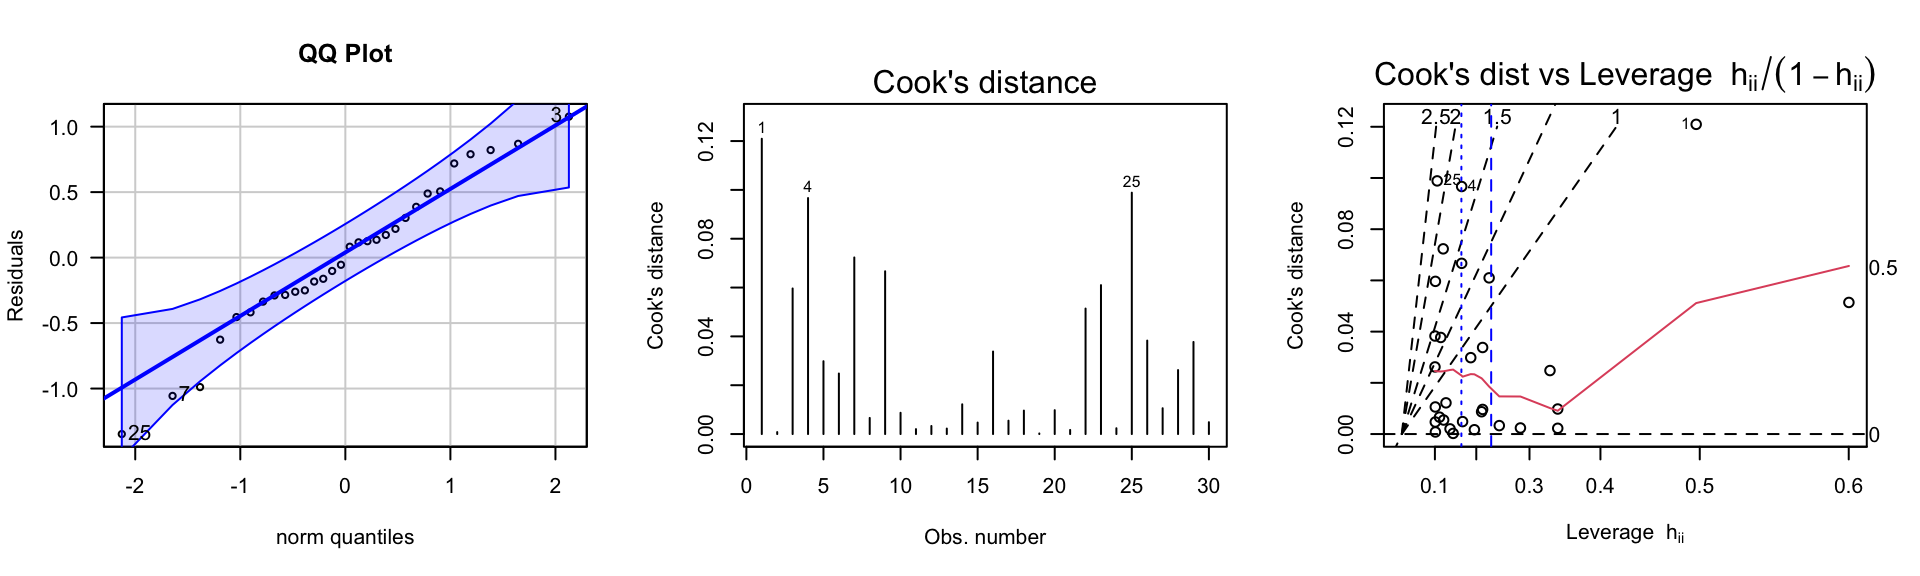
\includegraphics{ADA2_CL_14_ANCOVA_AbqHomePrices_files/figure-latex/unnamed-chunk-5-1} \end{center}

\begin{center}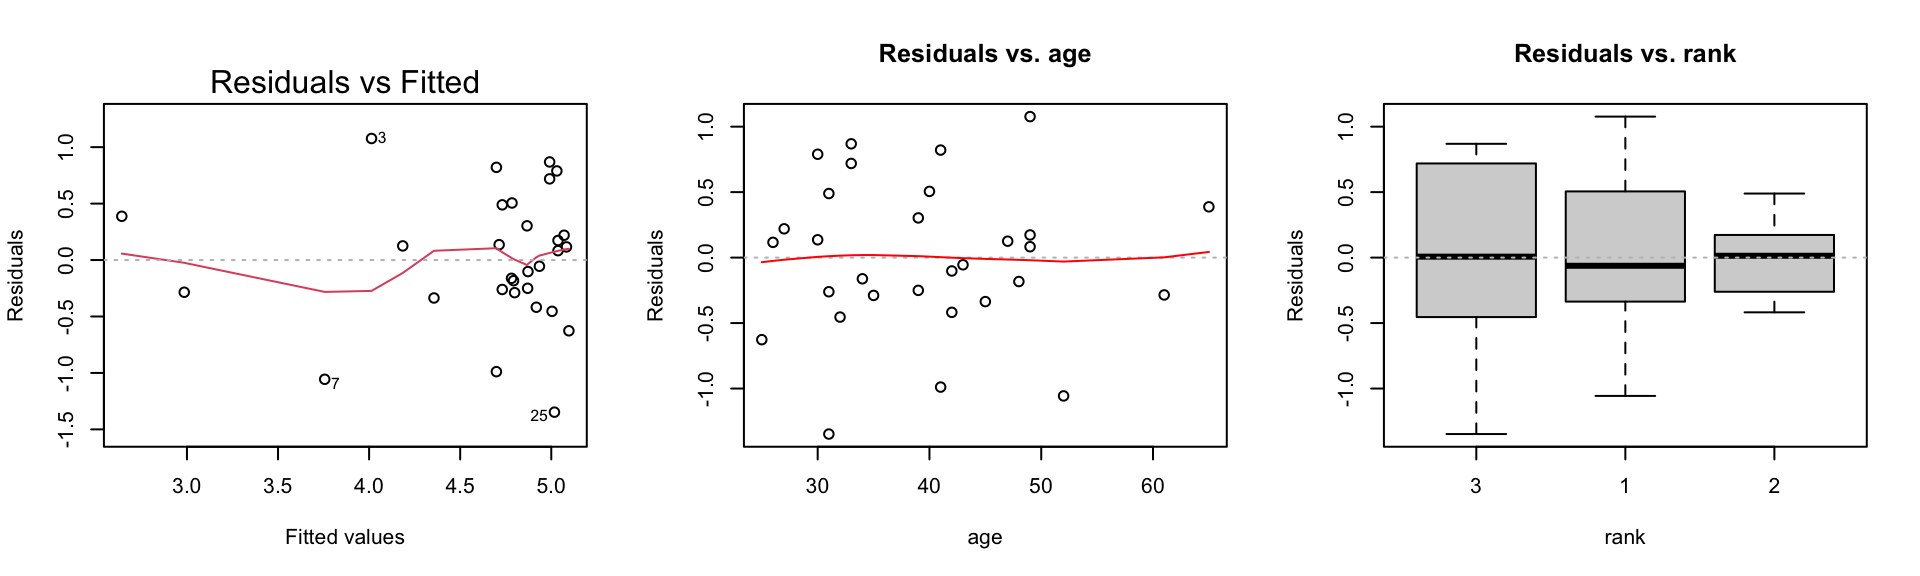
\includegraphics{ADA2_CL_14_ANCOVA_AbqHomePrices_files/figure-latex/unnamed-chunk-5-2} \end{center}

\begin{center}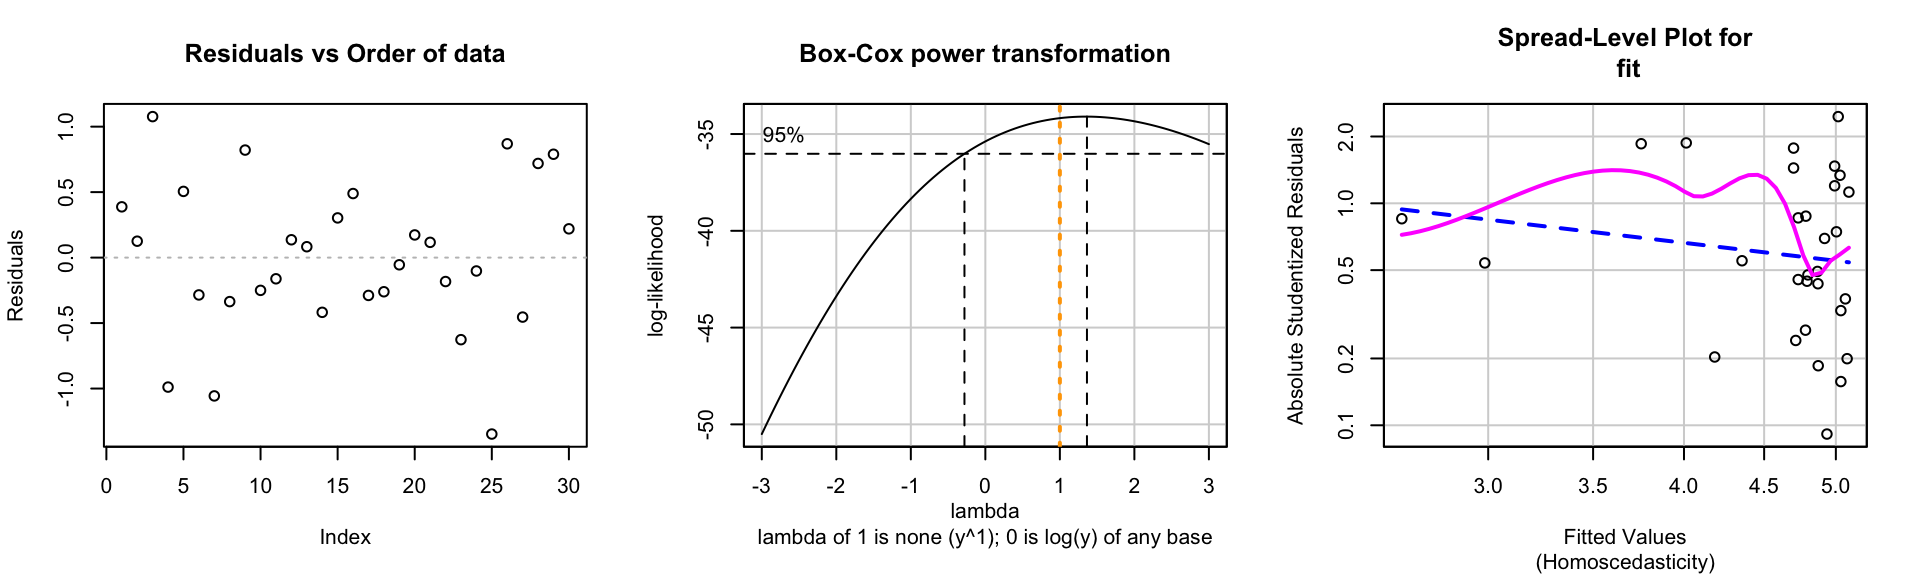
\includegraphics{ADA2_CL_14_ANCOVA_AbqHomePrices_files/figure-latex/unnamed-chunk-5-3} \end{center}

\begin{verbatim}
Non-constant Variance Score Test 
Variance formula: ~ fitted.values 
Chisquare = 1.593903, Df = 1, p = 0.20677
\end{verbatim}

\begin{center}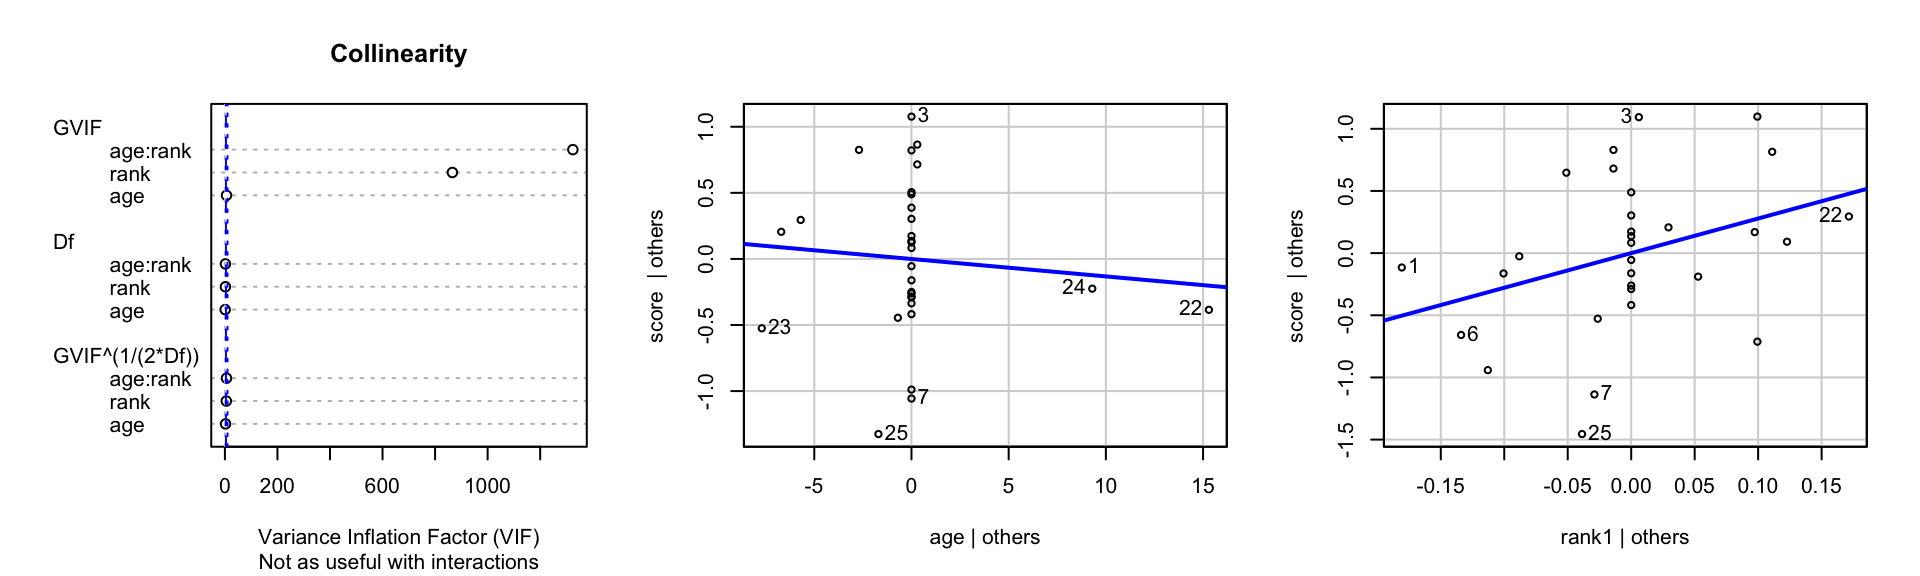
\includegraphics{ADA2_CL_14_ANCOVA_AbqHomePrices_files/figure-latex/unnamed-chunk-5-4} \end{center}

\begin{center}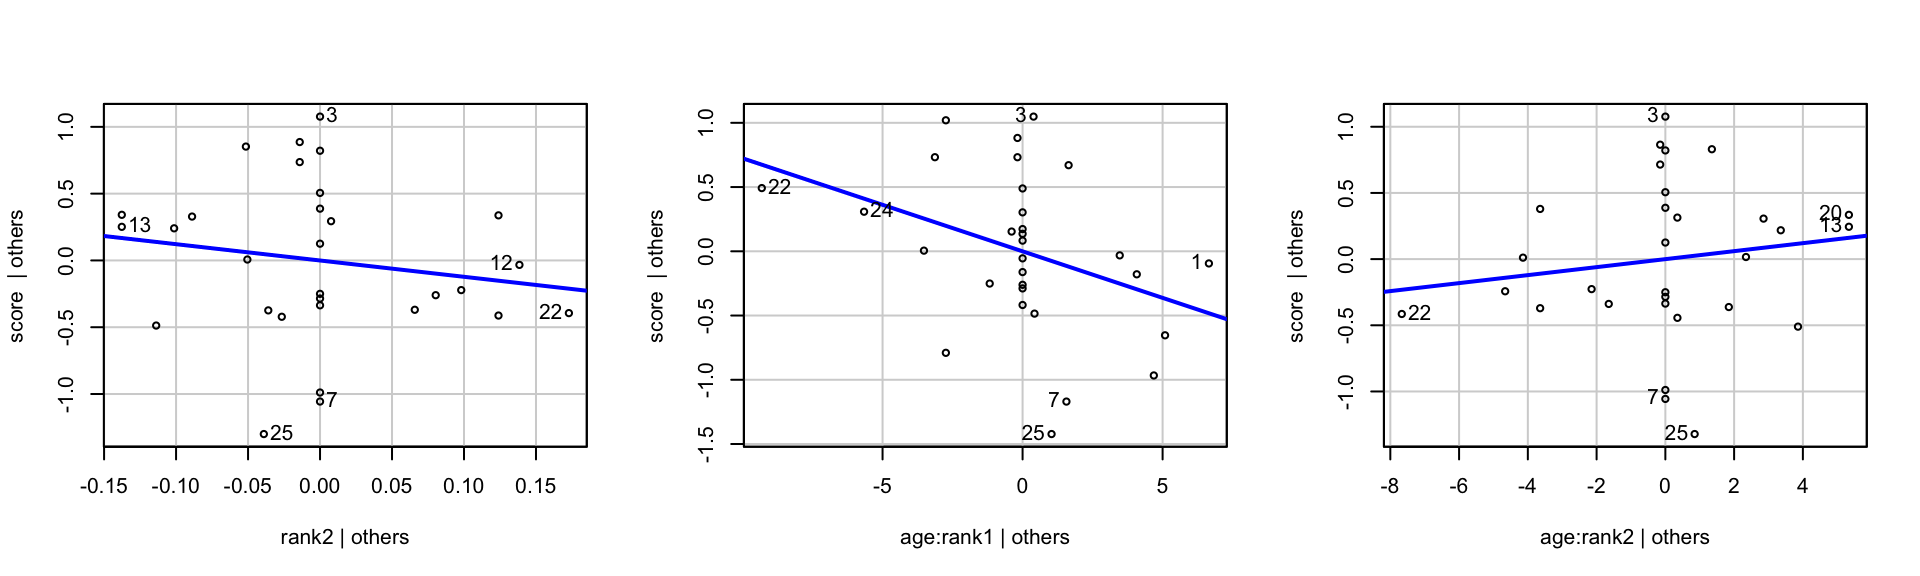
\includegraphics{ADA2_CL_14_ANCOVA_AbqHomePrices_files/figure-latex/unnamed-chunk-5-5} \end{center}

\begin{center}\includegraphics{ADA2_CL_14_ANCOVA_AbqHomePrices_files/figure-latex/unnamed-chunk-5-6} \end{center}

\begin{Shaded}
\begin{Highlighting}[]
\DocumentationTok{\#\# Remove influential observation}
\NormalTok{  dat\_abq }\OtherTok{\textless{}{-}}
\NormalTok{    dat\_abq }\SpecialCharTok{\%\textgreater{}\%}
    \FunctionTok{filter}\NormalTok{(}
\NormalTok{      YearBuilt\_1900 }\SpecialCharTok{\textless{}} \DecValTok{100}\NormalTok{, }
\NormalTok{      PriceListK }\SpecialCharTok{\textless{}} \DecValTok{539}\NormalTok{, }
\NormalTok{      DaysListed }\SpecialCharTok{\textless{}} \DecValTok{1000}\NormalTok{, }
\NormalTok{      Size\_sqft }\SpecialCharTok{\textless{}} \DecValTok{7000}
\NormalTok{    ) }

\NormalTok{mod1 }\OtherTok{\textless{}{-}} \FunctionTok{lm}\NormalTok{(logPriceList }\SpecialCharTok{\textasciitilde{}}\NormalTok{ Beds }\SpecialCharTok{+}\NormalTok{ Size\_sqft }\SpecialCharTok{+}\NormalTok{ DaysListed }\SpecialCharTok{+}\NormalTok{ YearBuilt\_1900 }\SpecialCharTok{+} \FunctionTok{I}\NormalTok{(YearBuilt\_1900}\SpecialCharTok{\^{}}\DecValTok{2}\NormalTok{), }
           \AttributeTok{data =}\NormalTok{ dat\_abq)}

\FunctionTok{e\_plot\_lm\_diagostics}\NormalTok{(mod1)}
\end{Highlighting}
\end{Shaded}

\begin{center}\includegraphics{ADA2_CL_14_ANCOVA_AbqHomePrices_files/figure-latex/unnamed-chunk-5-7} \end{center}

\begin{center}\includegraphics{ADA2_CL_14_ANCOVA_AbqHomePrices_files/figure-latex/unnamed-chunk-5-8} \end{center}

\begin{center}\includegraphics{ADA2_CL_14_ANCOVA_AbqHomePrices_files/figure-latex/unnamed-chunk-5-9} \end{center}

\begin{verbatim}
Non-constant Variance Score Test 
Variance formula: ~ fitted.values 
Chisquare = 0.2940893, Df = 1, p = 0.58761
\end{verbatim}

\begin{center}\includegraphics{ADA2_CL_14_ANCOVA_AbqHomePrices_files/figure-latex/unnamed-chunk-5-10} \end{center}

\begin{center}\includegraphics{ADA2_CL_14_ANCOVA_AbqHomePrices_files/figure-latex/unnamed-chunk-5-11} \end{center}

\begin{center}\includegraphics{ADA2_CL_14_ANCOVA_AbqHomePrices_files/figure-latex/unnamed-chunk-5-12} \end{center}

This looks pretty good. Adding a quadratic term for year built seems to
work. The 70s were really bad. Just awful.

\hypertarget{subset-data-for-model-building-and-prediction}{%
\subsection{Subset data for model building and
prediction}\label{subset-data-for-model-building-and-prediction}}

Create a subset of the data for building the model, and another subset
for prediction later on.

\begin{Shaded}
\begin{Highlighting}[]
\CommentTok{\# remove observations with NAs}
\NormalTok{dat\_abq }\OtherTok{\textless{}{-}}
\NormalTok{  dat\_abq }\SpecialCharTok{\%\textgreater{}\%}
  \FunctionTok{na.omit}\NormalTok{()}

\CommentTok{\# the data subset we will use to build our model}
\NormalTok{dat\_sub }\OtherTok{\textless{}{-}}
\NormalTok{  dat\_abq }\SpecialCharTok{\%\textgreater{}\%}
  \FunctionTok{filter}\NormalTok{(}
\NormalTok{    DaysListed }\SpecialCharTok{\textgreater{}} \DecValTok{0}
\NormalTok{  )}

\CommentTok{\# the data subset we will predict from our model}
\NormalTok{dat\_pred }\OtherTok{\textless{}{-}}
\NormalTok{  dat\_abq }\SpecialCharTok{\%\textgreater{}\%}
  \FunctionTok{filter}\NormalTok{(}
\NormalTok{    DaysListed }\SpecialCharTok{==} \DecValTok{0}
\NormalTok{  ) }\SpecialCharTok{\%\textgreater{}\%}
  \FunctionTok{mutate}\NormalTok{(}
    \CommentTok{\# the prices we hope to predict closely from our model}
    \AttributeTok{PriceListK\_true =}\NormalTok{ logPriceList}
    \CommentTok{\# set them to NA to predict them later}
\NormalTok{  , }\AttributeTok{PriceListK =} \ConstantTok{NA}
\NormalTok{  )}
\end{Highlighting}
\end{Shaded}

Scatterplot of the model-building subset.

\begin{Shaded}
\begin{Highlighting}[]
\CommentTok{\# }\AlertTok{NOTE}\CommentTok{, this plot takes a long time if you\textquotesingle{}re repeadly recompiling the document.}
\CommentTok{\# comment the "print(p)" line so save some time when you\textquotesingle{}re not evaluating this plot.}
\FunctionTok{library}\NormalTok{(GGally)}
\FunctionTok{library}\NormalTok{(ggplot2)}
\NormalTok{p }\OtherTok{\textless{}{-}}
  \FunctionTok{ggpairs}\NormalTok{(}
\NormalTok{    dat\_sub }\SpecialCharTok{\%\textgreater{}\%} \FunctionTok{select}\NormalTok{(}\SpecialCharTok{{-}}\NormalTok{id)}
\NormalTok{  , }\AttributeTok{mapping =}\NormalTok{ ggplot2}\SpecialCharTok{::}\FunctionTok{aes}\NormalTok{(}\AttributeTok{colour =}\NormalTok{ TypeSale, }\AttributeTok{alpha =} \FloatTok{0.5}\NormalTok{)}
\NormalTok{  , }\AttributeTok{lower =} \FunctionTok{list}\NormalTok{(}\AttributeTok{continuous =} \StringTok{"points"}\NormalTok{)}
\NormalTok{  , }\AttributeTok{upper =} \FunctionTok{list}\NormalTok{(}\AttributeTok{continuous =} \StringTok{"cor"}\NormalTok{)}
\NormalTok{  , }\AttributeTok{progress =} \ConstantTok{FALSE}
\NormalTok{  )}
\FunctionTok{print}\NormalTok{(p)}
\end{Highlighting}
\end{Shaded}

\begin{center}\includegraphics{ADA2_CL_14_ANCOVA_AbqHomePrices_files/figure-latex/unnamed-chunk-7-1} \end{center}

All the apartments appear to have only one bed, yet they are larger?
Something fishy there.

For both number of beds (houses only) and square footage, we see clear
positive relationships with listing price.

There may be an outlier in the number of days listed \ldots{} but it
wasn't apparent in the diagnostics, so I'm going to roll with it.

The log-transformed data look more normally distributed than the raw
data.

\hypertarget{solution-1}{%
\subsubsection{Solution}\label{solution-1}}

{[}answer{]}

Features of data:

\hypertarget{p-step-2-fit-full-two-way-interaction-model.}{%
\subsection{\texorpdfstring{\textbf{(2 p)} (Step 2) Fit full two-way
interaction
model.}{(2 p) (Step 2) Fit full two-way interaction model.}}\label{p-step-2-fit-full-two-way-interaction-model.}}

\emph{You'll revisit this section after each modification of the data
above.}

\textbf{Step 2:} Let's fit the full two-way interaction model and assess
the assumptions. However, some of the predictor variables are highly
correlated. Recall that the interpretation of a beta coefficient is
``the expected increase in the response for a 1-unit increase in \(x\)
with all other predictors held constant''. It's hard to hold one
variable constant if it's correlated with another variable you're
increasing. Therefore, we'll make a decision to retain some variables
but not others depending on their correlation values. (In the PCA
chapter, we'll see another strategy.)

Somewhat arbitrarily, let's exclude \texttt{Baths} (since highly
correlated with \texttt{Beds} and \texttt{Size\_sqft}). Let's also
exclude \texttt{LotSize} (since highly correlated with
\texttt{Size\_sqft}). Modify the code below. Notice that because
APARTMENTs don't have more than 1 Beds or Baths, those interaction terms
need to be excluded from the model; I show you how to do this manually
using the \texttt{update()} function.

Note that the formula below
\texttt{y\ \textasciitilde{}\ (x1\ +\ x2\ +\ x3)\^{}2} expands into all
main effects and two-way interactions.

\begin{Shaded}
\begin{Highlighting}[]
  \DocumentationTok{\#\# SOLUTION}
\NormalTok{dat\_sub }\OtherTok{\textless{}{-}}\NormalTok{ dat\_sub }\SpecialCharTok{\%\textgreater{}\%}
  \FunctionTok{filter}\NormalTok{(}\SpecialCharTok{!}\NormalTok{ id }\SpecialCharTok{\%in\%} \FunctionTok{c}\NormalTok{(}\DecValTok{59}\NormalTok{, }\DecValTok{74}\NormalTok{, }\DecValTok{75}\NormalTok{))}

\NormalTok{  lm\_full }\OtherTok{\textless{}{-}}
    \FunctionTok{lm}\NormalTok{(}
\NormalTok{      logPriceList }\SpecialCharTok{\textasciitilde{}}\NormalTok{ (TypeSale }\SpecialCharTok{+}\NormalTok{ Beds }\SpecialCharTok{+}\NormalTok{ logSizeSqft }\SpecialCharTok{+}\NormalTok{ DaysListed }\SpecialCharTok{+}\NormalTok{ YearBuilt\_1900)}\SpecialCharTok{\^{}}\DecValTok{2}
\NormalTok{    , }\AttributeTok{data =}\NormalTok{ dat\_sub}
\NormalTok{    )}
  \CommentTok{\#lm\_full \textless{}{-}}
  \CommentTok{\#  lm(}
  \CommentTok{\#    PriceListK \textasciitilde{} (Beds + Baths + Size\_sqft + LotSize + DaysListed + YearBuilt\_1900)\^{}2}
  \CommentTok{\#  , data = dat\_sub}
  \CommentTok{\#  )}
\NormalTok{  lm\_full}
\end{Highlighting}
\end{Shaded}

\begin{verbatim}
Call:
lm(formula = logPriceList ~ (TypeSale + Beds + logSizeSqft + 
    DaysListed + YearBuilt_1900)^2, data = dat_sub)

Coefficients:
                 (Intercept)                 TypeSaleHOUSE  
                   6.296e+00                     9.084e-01  
                        Beds                   logSizeSqft  
                  -3.532e-01                    -1.804e-01  
                  DaysListed                YearBuilt_1900  
                   1.681e-04                    -7.652e-02  
          TypeSaleHOUSE:Beds     TypeSaleHOUSE:logSizeSqft  
                          NA                    -2.058e-01  
    TypeSaleHOUSE:DaysListed  TypeSaleHOUSE:YearBuilt_1900  
                  -1.700e-04                     2.454e-04  
            Beds:logSizeSqft               Beds:DaysListed  
                   7.051e-02                     4.533e-05  
         Beds:YearBuilt_1900        logSizeSqft:DaysListed  
                   2.121e-03                    -1.814e-04  
  logSizeSqft:YearBuilt_1900     DaysListed:YearBuilt_1900  
                   1.996e-02                     7.739e-06  
\end{verbatim}

\begin{Shaded}
\begin{Highlighting}[]
  \FunctionTok{library}\NormalTok{(car)}
  \FunctionTok{try}\NormalTok{(}\FunctionTok{Anova}\NormalTok{(lm\_full, }\AttributeTok{type=}\DecValTok{3}\NormalTok{))}
\end{Highlighting}
\end{Shaded}

\begin{verbatim}
Error in Anova.III.lm(mod, error, singular.ok = singular.ok, ...) : 
  there are aliased coefficients in the model
\end{verbatim}

\begin{Shaded}
\begin{Highlighting}[]
  \DocumentationTok{\#\# Note that this doesn\textquotesingle{}t work because APARTMENTs only have 1 bed and 1 bath.}
  \DocumentationTok{\#\# There isn\textquotesingle{}t a second level of bed or bath to estimate the interaction.}
  \DocumentationTok{\#\# Therefore, remove those two terms}
\NormalTok{  lm\_full }\OtherTok{\textless{}{-}}
    \FunctionTok{update}\NormalTok{(}
\NormalTok{      lm\_full}
\NormalTok{    , . }\SpecialCharTok{\textasciitilde{}}\NormalTok{ . }\SpecialCharTok{{-}}\NormalTok{ TypeSale}\SpecialCharTok{:}\NormalTok{Beds}
\NormalTok{    )}
  \FunctionTok{library}\NormalTok{(car)}
  \FunctionTok{try}\NormalTok{(}\FunctionTok{Anova}\NormalTok{(lm\_full, }\AttributeTok{type=}\DecValTok{3}\NormalTok{))}
\end{Highlighting}
\end{Shaded}

\begin{tabular}{l|r|r|r|r}
\hline
  & Sum Sq & Df & F value & Pr(>F)\\
\hline
(Intercept) & 0.1244789 & 1 & 8.6120100 & 0.0041341\\
\hline
TypeSale & 0.0116744 & 1 & 0.8076904 & 0.3709415\\
\hline
Beds & 0.0105955 & 1 & 0.7330474 & 0.3939239\\
\hline
logSizeSqft & 0.0010728 & 1 & 0.0742184 & 0.7858471\\
\hline
DaysListed & 0.0000357 & 1 & 0.0024705 & 0.9604560\\
\hline
YearBuilt\_1900 & 0.0518451 & 1 & 3.5868741 & 0.0610991\\
\hline
TypeSale:logSizeSqft & 0.0065211 & 1 & 0.4511567 & 0.5033196\\
\hline
TypeSale:DaysListed & 0.0013675 & 1 & 0.0946101 & 0.7590296\\
\hline
TypeSale:YearBuilt\_1900 & 0.0000156 & 1 & 0.0010776 & 0.9738773\\
\hline
Beds:logSizeSqft & 0.0043809 & 1 & 0.3030930 & 0.5831655\\
\hline
Beds:DaysListed & 0.0006384 & 1 & 0.0441662 & 0.8339681\\
\hline
Beds:YearBuilt\_1900 & 0.0083134 & 1 & 0.5751605 & 0.4499816\\
\hline
logSizeSqft:DaysListed & 0.0003721 & 1 & 0.0257469 & 0.8728405\\
\hline
logSizeSqft:YearBuilt\_1900 & 0.0399569 & 1 & 2.7643964 & 0.0994835\\
\hline
DaysListed:YearBuilt\_1900 & 0.0047509 & 1 & 0.3286896 & 0.5677061\\
\hline
Residuals & 1.4598647 & 101 & NA & NA\\
\hline
\end{tabular}

\begin{Shaded}
\begin{Highlighting}[]
\DocumentationTok{\#\# Uncomment this line when you\textquotesingle{}re ready to assess the model assumptions}
\CommentTok{\# plot diagnostics}
\FunctionTok{e\_plot\_lm\_diagostics}\NormalTok{(lm\_full)}
\end{Highlighting}
\end{Shaded}

\begin{center}\includegraphics{ADA2_CL_14_ANCOVA_AbqHomePrices_files/figure-latex/unnamed-chunk-9-1} \end{center}

\begin{center}\includegraphics{ADA2_CL_14_ANCOVA_AbqHomePrices_files/figure-latex/unnamed-chunk-9-2} \end{center}

\begin{center}\includegraphics{ADA2_CL_14_ANCOVA_AbqHomePrices_files/figure-latex/unnamed-chunk-9-3} \end{center}

\begin{verbatim}
Non-constant Variance Score Test 
Variance formula: ~ fitted.values 
Chisquare = 0.3603047, Df = 1, p = 0.54834
\end{verbatim}

\begin{center}\includegraphics{ADA2_CL_14_ANCOVA_AbqHomePrices_files/figure-latex/unnamed-chunk-9-4} \end{center}

\begin{center}\includegraphics{ADA2_CL_14_ANCOVA_AbqHomePrices_files/figure-latex/unnamed-chunk-9-5} \end{center}

\begin{center}\includegraphics{ADA2_CL_14_ANCOVA_AbqHomePrices_files/figure-latex/unnamed-chunk-9-6} \end{center}

\begin{center}\includegraphics{ADA2_CL_14_ANCOVA_AbqHomePrices_files/figure-latex/unnamed-chunk-9-7} \end{center}

\begin{center}\includegraphics{ADA2_CL_14_ANCOVA_AbqHomePrices_files/figure-latex/unnamed-chunk-9-8} \end{center}

\begin{center}\includegraphics{ADA2_CL_14_ANCOVA_AbqHomePrices_files/figure-latex/unnamed-chunk-9-9} \end{center}

\begin{Shaded}
\begin{Highlighting}[]
\CommentTok{\# List the row numbers with id numbers}
\CommentTok{\#   The row numbers appear in the residual plots.}
\CommentTok{\#   The id number can be used to exclude values in code above.}
\NormalTok{dat\_sub }\SpecialCharTok{\%\textgreater{}\%} \FunctionTok{select}\NormalTok{(id) }\SpecialCharTok{\%\textgreater{}\%} \FunctionTok{print}\NormalTok{(}\AttributeTok{n =} \ConstantTok{Inf}\NormalTok{)}
\end{Highlighting}
\end{Shaded}

\begin{verbatim}
# A tibble: 116 x 1
       id
    <int>
  1     6
  2     7
  3     9
  4    10
  5    12
  6    13
  7    14
  8    15
  9    16
 10    17
 11    19
 12    20
 13    21
 14    22
 15    23
 16    24
 17    25
 18    26
 19    27
 20    28
 21    29
 22    30
 23    31
 24    33
 25    34
 26    35
 27    36
 28    38
 29    39
 30    40
 31    41
 32    42
 33    43
 34    44
 35    45
 36    46
 37    47
 38    48
 39    49
 40    51
 41    52
 42    53
 43    54
 44    55
 45    56
 46    57
 47    58
 48    60
 49    61
 50    62
 51    64
 52    65
 53    67
 54    68
 55    69
 56    70
 57    71
 58    72
 59    73
 60    76
 61    77
 62    78
 63    79
 64    81
 65    83
 66    84
 67    85
 68    86
 69    87
 70    88
 71    89
 72    91
 73    92
 74    94
 75    95
 76    97
 77    98
 78    99
 79   100
 80   101
 81   102
 82   103
 83   104
 84   105
 85   106
 86   108
 87   109
 88   110
 89   111
 90   112
 91   113
 92   114
 93   115
 94   116
 95   117
 96   118
 97   119
 98   121
 99   122
100   123
101   124
102   126
103   127
104   128
105   129
106   131
107   132
108   133
109   134
110   135
111   136
112   137
113   138
114   140
115   141
116   142
\end{verbatim}

After Step 2, interpret the residual plots. What are the primary issues
in the original model?

See discussion above. There were a lot of outliers influencing the data,
and the response needed a transformation. AFter removing outliers, the
data don't seem all that normally distributed anymore. They're pretty
close though, so we'll just keep moving along.

\hypertarget{solution-2}{%
\subsubsection{Solution}\label{solution-2}}

{[}answer{]}

\hypertarget{p-step-5-model-selection-check-model-assumptions.}{%
\subsection{\texorpdfstring{\textbf{(2 p)} (Step 5) Model selection,
check model
assumptions.}{(2 p) (Step 5) Model selection, check model assumptions.}}\label{p-step-5-model-selection-check-model-assumptions.}}

Using \texttt{step(...,\ direction="both")} with the BIC criterion,
perform model selection.

\hypertarget{solution-3}{%
\subsubsection{Solution}\label{solution-3}}

\begin{Shaded}
\begin{Highlighting}[]
\DocumentationTok{\#\# BIC}
\CommentTok{\# option: test="F" includes additional information}
\CommentTok{\#           for parameter estimate tests that we\textquotesingle{}re familiar with}
\CommentTok{\# option: for BIC, include k=log(nrow( [data.frame name] ))}
\NormalTok{lm\_red\_BIC }\OtherTok{\textless{}{-}}
  \FunctionTok{step}\NormalTok{(}
\NormalTok{    lm\_full}
\NormalTok{  , }\AttributeTok{direction =} \StringTok{"both"}
\NormalTok{  , }\AttributeTok{test =} \StringTok{"F"}
\NormalTok{  , }\AttributeTok{trace =} \DecValTok{0}
\NormalTok{  , }\AttributeTok{k =} \FunctionTok{log}\NormalTok{(}\FunctionTok{nrow}\NormalTok{(dat\_sub))}
\NormalTok{  )}
\NormalTok{lm\_final }\OtherTok{\textless{}{-}}\NormalTok{ lm\_red\_BIC}
\NormalTok{lm\_red\_BIC}
\end{Highlighting}
\end{Shaded}

\begin{verbatim}
Call:
lm(formula = logPriceList ~ TypeSale + logSizeSqft + YearBuilt_1900, 
    data = dat_sub)

Coefficients:
   (Intercept)   TypeSaleHOUSE     logSizeSqft  YearBuilt_1900  
      2.451636        0.215648        0.881960       -0.004028  
\end{verbatim}

\begin{Shaded}
\begin{Highlighting}[]
\DocumentationTok{\#\# Uncomment this line when you\textquotesingle{}re ready to assess the model assumptions}
\CommentTok{\# plot diagnostics}
\FunctionTok{e\_plot\_lm\_diagostics}\NormalTok{(lm\_final)}
\end{Highlighting}
\end{Shaded}

\begin{center}\includegraphics{ADA2_CL_14_ANCOVA_AbqHomePrices_files/figure-latex/unnamed-chunk-11-1} \end{center}

\begin{center}\includegraphics{ADA2_CL_14_ANCOVA_AbqHomePrices_files/figure-latex/unnamed-chunk-11-2} \end{center}

\begin{center}\includegraphics{ADA2_CL_14_ANCOVA_AbqHomePrices_files/figure-latex/unnamed-chunk-11-3} \end{center}

\begin{verbatim}
Non-constant Variance Score Test 
Variance formula: ~ fitted.values 
Chisquare = 3.055127, Df = 1, p = 0.080483
\end{verbatim}

\begin{center}\includegraphics{ADA2_CL_14_ANCOVA_AbqHomePrices_files/figure-latex/unnamed-chunk-11-4} \end{center}

\begin{center}\includegraphics{ADA2_CL_14_ANCOVA_AbqHomePrices_files/figure-latex/unnamed-chunk-11-5} \end{center}

So, the model that included a quadratic term for year built was selected
by stepwise regression, but it resulted in a dubious, complex model. I
simplified things by removing the quadratic, leading to an additive
model with good diagnostics. There do not appear to be outliers, the
residuals are (mostly) normally distributed, and variance is well
stabilized.

\hypertarget{p-step-6-plot-final-model-interpret-coefficients.}{%
\subsection{\texorpdfstring{\textbf{(4 p)} (Step 6) Plot final model,
interpret
coefficients.}{(4 p) (Step 6) Plot final model, interpret coefficients.}}\label{p-step-6-plot-final-model-interpret-coefficients.}}

If you arrived at the same model I did, then the code below will plot
it. Eventually (after Step 7), the fitted model equations will describe
the each dwelling \texttt{TypeSale} and interpret the coefficients.

\begin{center}\includegraphics{ADA2_CL_14_ANCOVA_AbqHomePrices_files/figure-latex/unnamed-chunk-12-1} \end{center}

\begin{Shaded}
\begin{Highlighting}[]
\FunctionTok{library}\NormalTok{(car)}
\CommentTok{\#Anova(lm\_final, type=3)}
\FunctionTok{summary}\NormalTok{(lm\_final)}
\end{Highlighting}
\end{Shaded}

\begin{verbatim}
Call:
lm(formula = logPriceList ~ TypeSale + logSizeSqft + YearBuilt_1900, 
    data = dat_sub)

Residuals:
     Min       1Q   Median       3Q      Max 
-0.43211 -0.07393  0.01398  0.06793  0.31249 

Coefficients:
                Estimate Std. Error t value Pr(>|t|)    
(Intercept)     2.451636   0.244447  10.029  < 2e-16 ***
TypeSaleHOUSE   0.215648   0.030189   7.143 9.78e-11 ***
logSizeSqft     0.881960   0.076863  11.474  < 2e-16 ***
YearBuilt_1900 -0.004028   0.001307  -3.082  0.00259 ** 
---
Signif. codes:  0 '***' 0.001 '**' 0.01 '*' 0.05 '.' 0.1 ' ' 1

Residual standard error: 0.1193 on 112 degrees of freedom
Multiple R-squared:  0.5507,    Adjusted R-squared:  0.5386 
F-statistic: 45.76 on 3 and 112 DF,  p-value: < 2.2e-16
\end{verbatim}

Fitted model equation is \$\$ \widehat{\log(\textrm{PriceList})} = 2.45
+ 0.216 \times \text{I}(TypeSale = House) + 0.882 \times LogSqFt - .004
\times YearBuilt

\$\$

\hypertarget{solution-4}{%
\subsubsection{Solution}\label{solution-4}}

After Step 7, return and intepret the model coefficients above.

The intercept isn't worth interpreting, since it's relevant when Size
(sqft) is 0, a ridiculous and terrifying idea

The significant effect of TypeSale indicates that houses list for higher
prices than apartment. The significant effect of logSizeSqft indicates a
positive relationship between listing price and size for both apartments
and houses. Lastly, the significant negative relationship with YearBuilt
indicates older houses list for higher prices.

\hypertarget{p-step-7-transform-predictors.}{%
\subsection{\texorpdfstring{\textbf{(2 p)} (Step 7) Transform
predictors.}{(2 p) (Step 7) Transform predictors.}}\label{p-step-7-transform-predictors.}}

We now have enough information to see that a transformation of a
predictor can be useful. See the curvature with \texttt{Size\_sqft}?
This is one of the headaches of regression modelling, \emph{everything
depends on everything else} and you learn as you go. Return to the top
and transform \texttt{Size\_sqft} and \texttt{LotSize}.

A nice feature of this transformation is that the model interaction goes
away. Our interpretation is now on the log scale, but it's a simpler
model.

I don't know how to get points here. I did it.

\hypertarget{p-step-8-predict-new-observations-interpret-models-predictive-ability.}{%
\subsection{\texorpdfstring{\textbf{(4 p)} (Step 8) Predict new
observations, interpret model's predictive
ability.}{(4 p) (Step 8) Predict new observations, interpret model's predictive ability.}}\label{p-step-8-predict-new-observations-interpret-models-predictive-ability.}}

Using the \texttt{predict()} function, we'll input the data we held out
to predict earlier, and use our final model to predict the
\texttt{PriceListK} response. Note that \texttt{10\^{}lm\_pred} is the
table of values on the scale of ``thousands of dollars''.

Interpret the predictions below the output.

How well do you expect this model to predict? Justify your answer.

\begin{Shaded}
\begin{Highlighting}[]
\CommentTok{\# predict new observations, convert to data frame}
\NormalTok{lm\_pred }\OtherTok{\textless{}{-}}
  \FunctionTok{as.data.frame}\NormalTok{(}
    \FunctionTok{predict}\NormalTok{(}
\NormalTok{      lm\_final}
\NormalTok{    , }\AttributeTok{newdata =}\NormalTok{ dat\_pred}
\NormalTok{    , }\AttributeTok{interval =} \StringTok{"prediction"}
\NormalTok{    )}
\NormalTok{  ) }\SpecialCharTok{\%\textgreater{}\%}
  \FunctionTok{mutate}\NormalTok{(}
    \CommentTok{\# add column of actual list prices}
    \AttributeTok{PriceListK =}\NormalTok{ dat\_pred}\SpecialCharTok{$}\NormalTok{PriceListK\_true}
\NormalTok{  )}
\NormalTok{lm\_pred}
\end{Highlighting}
\end{Shaded}

\begin{tabular}{r|r|r|r}
\hline
fit & lwr & upr & PriceListK\\
\hline
5.197594 & 4.959557 & 5.435631 & 5.271609\\
\hline
5.258627 & 5.015824 & 5.501430 & 5.484300\\
\hline
5.135546 & 4.885871 & 5.385222 & 5.387390\\
\hline
\end{tabular}

\begin{Shaded}
\begin{Highlighting}[]
\CommentTok{\# on "thousands of dollars" scale}
\DecValTok{10}\SpecialCharTok{\^{}}\NormalTok{lm\_pred}
\end{Highlighting}
\end{Shaded}

\begin{tabular}{r|r|r|r}
\hline
fit & lwr & upr & PriceListK\\
\hline
157613.8 & 91108.19 & 272665.9 & 186900\\
\hline
181395.8 & 103710.81 & 317271.1 & 305000\\
\hline
136630.1 & 76890.25 & 242784.8 & 244000\\
\hline
\end{tabular}

\begin{Shaded}
\begin{Highlighting}[]
\CommentTok{\# attributes of the three predicted observations}
\NormalTok{dat\_pred }\SpecialCharTok{\%\textgreater{}\%} \FunctionTok{print}\NormalTok{(}\AttributeTok{n =} \ConstantTok{Inf}\NormalTok{, }\AttributeTok{width =} \ConstantTok{Inf}\NormalTok{)}
\end{Highlighting}
\end{Shaded}

\begin{verbatim}
# A tibble: 3 x 10
     id TypeSale   Beds Size_sqft DaysListed YearBuilt_1900 logPriceList
  <int> <fct>     <dbl>     <dbl>      <dbl>          <dbl>        <dbl>
1     1 HOUSE         3      1305          0             54         5.27
2     2 APARTMENT     1      2523          0             48         5.48
3     3 APARTMENT     1      2816          0             89         5.39
  logSizeSqft PriceListK PriceListK_true
        <dbl> <lgl>                <dbl>
1        3.12 NA                    5.27
2        3.40 NA                    5.48
3        3.45 NA                    5.39
\end{verbatim}

\hypertarget{solution-5}{%
\subsubsection{Solution}\label{solution-5}}

It didn't do so great, but we don't have a benchmark in any case.
Personally, I think we ought not to have chosen the 0 days listed
properties, which typically will list for higher than older properties.
Indeed, we see that we are under-predicting the property listing values
here. A better approach would be to randomly sample a handfull (20\%?)
of properties for prediction, and use DaysListed as a feature in the
prediction process.

\end{document}
